% !TEX program = xelatex
% Standalone CVPR-style supplementary material.
\documentclass[10pt,twocolumn,letterpaper]{article}
\usepackage[review]{cvpr}
% Portable Times-compatible Unicode fonts; CVPR geometry is unchanged.
\usepackage{iftex}
\ifXeTeX
  \usepackage{fontspec}
  \setmainfont{texgyretermes-regular.otf}[
    BoldFont=texgyretermes-bold.otf,ItalicFont=texgyretermes-italic.otf,
    BoldItalicFont=texgyretermes-bolditalic.otf]
  \setsansfont{texgyreheros-regular.otf}[
    BoldFont=texgyreheros-bold.otf,ItalicFont=texgyreheros-italic.otf,
    BoldItalicFont=texgyreheros-bolditalic.otf]
  \setmonofont{texgyrecursor-regular.otf}[
    BoldFont=texgyrecursor-bold.otf,ItalicFont=texgyrecursor-italic.otf,
    BoldItalicFont=texgyrecursor-bolditalic.otf]
\fi

\usepackage{booktabs}
\usepackage{graphicx,placeins,multirow,float}
\usepackage{amsmath,amssymb}
\definecolor{cvprblue}{rgb}{0.21,0.49,0.74}
\usepackage[pagebackref,breaklinks,colorlinks,allcolors=cvprblue]{hyperref}
\def\paperID{*****}
\def\confName{CVPR}
\def\confYear{2027}
\title{DriveCompose: Compositional Generative Reconstruction of Driving Scenes via Joint Completion}
\author{Anonymous CVPR Submission}
\begin{document}
% Allow related supplementary result tables to share a page without changing fonts or geometry.
\setcounter{topnumber}{5}
\setcounter{dbltopnumber}{5}
\setcounter{totalnumber}{10}
\renewcommand{\topfraction}{0.9}
\renewcommand{\dbltopfraction}{0.9}
\renewcommand{\textfraction}{0.05}
\renewcommand{\floatpagefraction}{0.75}
\renewcommand{\dblfloatpagefraction}{0.75}
% Keep lineno's column marker before the column contents (legacy wrapper).
% The inherited CVPR style with this TeX version places the hook marker after
% the contents in the standalone supplementary title path.
\makeatletter
\RemoveFromHook{build/column/before}[lineno]
\let\DCoriginalmakecol\@makecol
\def\@makecol{%
  \DCoriginalmakecol
  \setbox\@outputbox\vbox{%
    \boxmaxdepth\@maxdepth
    \protected@write\@auxout{}{%
      \string\def\string\@LN@column{\if@firstcolumn1\else2\fi}}%
    \box\@outputbox}}
\let\@LN@makecol\@makecol
\makeatother

\maketitlesupplementary
\appendix
\renewcommand{\thetable}{S\arabic{table}}
\renewcommand{\theequation}{S\arabic{equation}}
\renewcommand{\thefigure}{S\arabic{figure}}
\section{Cross-dataset generalization}
\label{sec:supp-generalization}
We evaluate zero-shot transfer of Waymo-trained checkpoints on 150 nuScenes validation scenes. Each scene supplies one fixed, continuous 20-frame clip from FRONT, FRONT\_LEFT, and FRONT\_RIGHT. Native camera timestamps give a clip duration of approximately 1.67 s. Inputs at $\{0,5,10,15\}$ leave 16 targets: 150 clips contain 1,800 context and 7,200 target images, including 5,400 interpolation and 1,800 extrapolation targets. Outputs are $240\times160$.

The supplied camera and actor states and shared state adapters match the Waymo conditions. All networks, codecs, and normalization parameters remain frozen, without target-domain training or scene adaptation. Table~\ref{tab:generalization} reports means and sample SDs across training seeds. Ours improves over DGGT by 1.16 dB PSNR and 0.009 SSIM, supporting reconstruction transfer under these fixed conditions. Each dataset retains its native camera timing.

\begin{table}[!htbp]
\centering\small
\setlength{\tabcolsep}{4pt}
\caption{Zero-shot reconstruction on nuScenes. Mean $\pm$ training-seed SD.}
\label{tab:generalization}
\begin{tabular}{@{}lcc@{}}
\toprule
Method & PSNR $\uparrow$ & SSIM $\uparrow$ \\
\midrule
STORM & 17.77 $\pm$ 0.12 & 0.669 $\pm$ 0.003 \\
DGGT & 25.31 $\pm$ 0.08 & 0.794 $\pm$ 0.002 \\
StreetForward & 23.17 $\pm$ 0.10 & 0.712 $\pm$ 0.003 \\
Ours & \textbf{26.47 $\pm$ 0.07} & \textbf{0.803 $\pm$ 0.002} \\
\bottomrule
\end{tabular}
\end{table}

\section{Training details}
\label{sec:supp-training}

Learning is divided into four stages so that the completion target has a stable meaning. Recovery determines the evidence and support, the codec defines its latent coordinates, and the completion network learns a distribution over the missing codes. The last stage adapts this distribution to real observations without changing the representation it predicts.

\paragraph{Data and splits.}
Counts in Table~\ref{tab:data-splits} include only data passing quality checks. The original Waymo training set is divided into 740 training and 58 development sequences; the 58 development sequences select checkpoints, and the 202 validation sequences are used for testing. Synthetic maps, base vehicle models, and human identities are separated by source asset. Texture variants of a vehicle and clothing/motion variants of a human remain in one split. Real logs are deduplicated and separated by road segment, continuous capture, and identifiable actors. Completeness refers to geometry, materials, and motion bindings within the finite query support.

\begin{table*}[!t]
\centering\small
\setlength{\tabcolsep}{4pt}
\caption{Data and supervision. Scene maps and independent assets are split by source identity.}
\label{tab:data-splits}
\begin{tabular}{@{}lrrrp{0.47\textwidth}@{}}
\toprule
Data & Train & Dev. & Test & Supervision \\
\midrule
Waymo sequences & 740 & 58 & 202 & RGB, calibration, ego poses, LiDAR, vehicle boxes and tracks \\
Synthetic scenes & 10,000 & 1,000 & 1,000 & Geometry, materials, depth, semantics, instances and actor states \\
Synthetic maps & 80 & 10 & 10 & Static background geometry and road structure \\
Vehicle assets & 10,000 & 1,000 & 1,000 & Canonical geometry, materials, dimensions and rigid frames \\
Human identities & 2,500 & 250 & 250 & Shape, texture, template, skeleton, skinning and joint states \\
\bottomrule
\end{tabular}
\end{table*}


\paragraph{Complete targets on a fixed layout.}
Partial input establishes $\mathcal Q$. Both branches use the same query positions, scales, types, order, component ownership, and human bindings, following the block order and within-block indices of \texttt{QueryBundle.blocks}. Complete meshes are queried on this fixed support. For each non-sky query, the owning component's mesh is expressed in the query frame and intersected with its cell $B_i$. Positive-area triangle intersections supply surface targets. A cell with no intersecting surface receives a surface-free target after asset completeness checks.

For an intersecting triangle fragment $f$ of area $A_f$, we draw
\begin{equation}
n_f=\max\!\left(1,\left\lceil\frac{64A_f}{\delta_{\min}^{\,2}}\right\rceil\right)
\label{eq:target-samples}
\end{equation}
deterministic area samples, where $\delta_{\min}$ is the smallest cell side. Asset, query, and triangle indices determine sample locations. We render RGB, camera-axis depth, instance identity, and triangle identity using original materials and fixed illumination. Eight azimuths and three elevations form the base views. Local isolated views cover remaining fragments, providing features for surfaces occluded in the base views.

The Stage 1 visual encoder, frozen after recovery training, maps rendered RGB to 128-dimensional features. At each surface sample, we extract these features and append its normalized depth residual relative to the query center, clipped to $[-1,1]$. We first average valid views of each sample with observation weights, then aggregate samples by fragment area to obtain $\mathbf h_i^{\rm full}\in\mathbb R^{129}$. The partial branch retains query-center projection and visibility-weighted aggregation.

Surface-free cells use a 129-dimensional zero feature and explicit zero-opacity supervision. Surface-free targets describe the absence of mesh surface; free-space labels are supplied by observed rays. Sky targets come from the complete environment map with zero depth residual. Both branches share the visual feature basis, input format, and type-specific codec. The target code is
\begin{equation}
\mathbf z_{1,i}=E_{k_i}([\mathbf h_i^{\rm full};\mathbf q_i;\boldsymbol\delta_i])
\in\mathbb R^{128}.
\label{eq:complete-code}
\end{equation}
The 135-dimensional input passes through a $135\rightarrow128\rightarrow128$ MLP and LayerNorm. Biases allow a zero feature to encode a nonzero latent. Hard projection separately enforces zero free-space codes during completion.

\begin{table*}[t]
\centering\small
\caption{Network and support configuration. Observed anchors and canonical human-template queries augment the base grids.}
\label{tab:network-config}
\begin{tabular}{@{}lp{0.70\textwidth}@{}}
\toprule
Module & Configuration \\
\midrule
Visual recovery & Width 128; patch size 16; 4 heads; 1 image-attention layer and 2 cross-view/time-summary layers \\
Identity and human state & 24 identity slots; 10-dimensional shape code; 17-joint interface \\
Query features and latents & Feature dimension 129; latent dimension 128; type-specific $135\rightarrow128\rightarrow128$ encoders with LayerNorm \\
Completion network & Width 128; 4 layers; 4 heads; 16 memory tokens \\
Gaussian decoding & 4 children per query; 23 outputs per child, including 12 appearance parameters \\
Directional appearance & Constant RGB and three local directional coefficients per channel \\
Base supports & Background $20\times12\times6$; rigid $8\times4\times4$; sky $4\times4$ per cubemap face \\
Sampling & 24 explicit Euler steps with observed-code restoration and free-space clearing after each step \\
\bottomrule
\end{tabular}
\end{table*}

\paragraph{Stage 1: visual recovery.}
Real training logs and synthetic scenes supervise the image encoder, geometry heads, identity slots, and state heads. Real depth comes from training LiDAR, and vehicle states come from annotations. Confidence-weighted real semantic and human-joint auxiliary labels complement synthetic shape, skeleton, binding, and joint supervision. One trajectory-level matching assigns slots to identities and is reused across timestamps. Confidence is trained or calibrated against depth, occlusion, and reprojection reliability. Table~\ref{tab:recovery-weights} lists the loss weights.

\begin{table}[t]
\centering\small
\caption{Stage 1 supervision weights.}
\label{tab:recovery-weights}
\begin{tabular}{@{}lrlr@{}}
\toprule
Loss & Weight & Loss & Weight \\
\midrule
Depth & 1.0 & Root rotation & 0.2 \\
Normals & 0.2 & Dimensions & 0.1 \\
Semantics & 0.1 & Human shape & 0.1 \\
Instances & 0.1 & Joints & 0.2 \\
Root translation & 0.5 & Confidence & 0.1 \\
\bottomrule
\end{tabular}
\end{table}

\paragraph{Stage 2: latent representation fitting.}
With recovery frozen, we train the codec on synthetic scenes and complete assets, together with real RGB, depth, and silhouette observations. The objective is
\begin{align}
\mathcal L_2={}&\mathcal L_{\rm rgb}+0.1\mathcal L_{\rm depth}
+0.2\mathcal L_{\rm silhouette}\nonumber\\
&+0.05\mathcal L_{\rm empty}+0.001\mathcal L_{\rm scale}.
\label{eq:codec-loss}
\end{align}
For rendered RGB $\widehat{\mathbf I}$ and depth $\widehat d$, the observation losses are masked L1 means,
\begin{align}
\mathcal L_{\rm rgb}&=\langle\|\widehat{\mathbf I}-\mathbf I\|_1/3\rangle_{\Omega_I},\\
\mathcal L_{\rm depth}&=\langle|\widehat d-d|\rangle_{\Omega_d}.
\label{eq:reconstruction-loss}
\end{align}
Here $\langle\ell\rangle_\Omega$ averages valid elements. Surface-free cells receive squared-opacity loss $\mathcal L_{\rm empty}$, alongside silhouette supervision and Gaussian-scale regularization. At the end of Stage 2, we freeze recovery and the codec and encode fixed complete targets $\mathbf z_1$ for prior learning.

\paragraph{Stage 3: completion-prior learning.}
The GCM learns the unknown-query flow-matching objective in Eq.~(9) of the main paper. Every unknown query in an accepted synthetic sample has valid geometry, appearance, and binding targets. Samples with an invalid unknown target are excluded from this stage; the loss selector $s_i$ operates within valid targets. Complete scenes provide cross-component context, and complete assets supply object geometry and appearance. Conditioning masks simulate contiguous unseen surfaces, background holes, long occlusions, short tracks, and uneven camera coverage. Pose, instance, and confidence perturbations expose the generator to recovery errors.

\paragraph{Stage 4: adaptation through rendering.}
We differentiate through flow integration, decoding, and rendering to update only the GCM. Complete synthetic samples and real logs from the 740 training sequences are mixed at $1{:}3$. The objective is
\begin{align}
\mathcal L_4={}&\mathcal L_{\rm flow}+\mathcal L_{\rm rgb}
+0.1\mathcal L_{\rm depth}+0.05\mathcal L_{\rm free}\nonumber\\
&+0.1\mathcal L_{\rm ground}+0.1\mathcal L_{\rm contact}
+0.1\mathcal L_{\rm penetration}.
\label{eq:adaptation}
\end{align}
The flow term uses complete synthetic samples; each observation or geometry term uses samples carrying its required supervision. Every term is averaged over its own valid elements. With accumulated free-ray opacity $a_r$, foot signed distance $d_f$ positive above ground, contacting feet $\Omega_c$, and penetration depth $d_p$ positive inside another actor, the geometry terms are
\begin{align}
\mathcal L_{\rm free}&=\langle a_r^2\rangle,&
\mathcal L_{\rm ground}&=\langle[-d_f]_+^2\rangle,\nonumber\\
\mathcal L_{\rm contact}&=\langle|d_f|\rangle_{\Omega_c},&
\mathcal L_{\rm penetration}&=\langle[d_p]_+^2\rangle,
\end{align}
where $[x]_+=\max(x,0)$. Frozen decoding and hard code restoration preserve the observed anchors.

\paragraph{Optimization and inference.}
Table~\ref{tab:training-schedule} gives the four-stage schedule. Training uses eight A100 80 GB GPUs, FP16, and AdamW with $\beta=(0.9,0.95)$ and weight decay 0.01. Each stage uses warmup followed by cosine learning-rate decay. The 58 development sequences select checkpoints; the 202 validation sequences form the test set. The four stages total 287,360 updates and 1,001.5 GPU hours, including method-specific target preprocessing. Stage costs are 278.6, 184.3, 326.9, and 211.7 GPU hours. Three GCM training seeds share recovery and the codec, giving a combined cost of 2,078.7 GPU hours. The w/o CCM control reuses Stages 1--2 and retrains Stages 3--4 with the same budget. The deterministic w/o GCM control uses the fixed recovery module and codec.

At inference, the log is encoded once. Its query layout and observed codes remain fixed throughout 24 Euler steps, after which type-specific decoders produce assets for repeated state composition.

\begin{table*}[t]
\centering\small
\caption{Four-stage training schedule. R: recovery; C: codec; G: GCM. $D_R$: real training logs; $D_S$: synthetic scenes; $D_A$: complete assets. Batch sizes are global.}
\label{tab:training-schedule}
\begin{tabular}{@{}lllc rrr@{}}
\toprule
Stage & Updated & Frozen & Data & Updates & Batch & Initial LR \\
\midrule
Visual recovery & R & -- & $D_R,D_S$ & 86,208 & 32 & $2\times10^{-4}$ \\
Latent fitting & C & R & $D_S,D_A,D_R$ & 57,472 & 32 & $3\times10^{-4}$ \\
Completion prior & G & R, C & Complete $D_S,D_A$ & 114,944 & 32 & $10^{-4}$ \\
Rendering adaptation & G & R, C & $D_S:D_R=1:3$ & 28,736 & 8 & $3\times10^{-5}$ \\
\bottomrule
\end{tabular}
\end{table*}

\section{Scene composition and checking details}
\label{sec:supp-composition}

\paragraph{State-driven rendering.}

At online step $k$, state $s_k$ specifies the ego pose, active assets, vehicle transforms, and human root and joint poses. A vehicle's Gaussian center and covariance transform as

\begin{equation}
\boldsymbol\mu^w=\mathbf R\boldsymbol\mu^a+\mathbf t,
\qquad
\boldsymbol\Sigma^w=\mathbf R\boldsymbol\Sigma^a\mathbf R^\top.
\label{eq:rigid}
\end{equation}

For humans, the weighted skinning transform is $\mathbf A_i=\sum_j w_{ij}\mathbf P_j\mathbf B_j^{-1}$, where $\mathbf B_j$ and $\mathbf P_j$ are rest and current global joints in the root frame. The transformed center is $\bar{\boldsymbol\mu}_i^w=\mathbf T^w_h\mathbf A_i\bar{\boldsymbol\mu}_i^h$. The combined local linear map $\mathbf J_i$ gives covariance $\mathbf J_i\boldsymbol\Sigma_i\mathbf J_i^\top$. Its inverse $\mathbf J_i^{-1}$ maps viewing directions into the canonical frame; the direction is normalized before appearance evaluation. Nearly singular skinning transforms are rejected. The root pose controls overall placement, while the root joint retains its rest transform.

The renderer composites the background, active assets, and valid sky. External policy and dynamics can advance the state:

\begin{align}
o_k&=\mathcal R(\operatorname{Compose}(\mathcal W,s_k),\mathcal C_k),\\
s_{k+1}&=F_{\rm dyn}(s_k,\pi(o_k),\Delta t).
\label{eq:simulation}
\end{align}

Resetting or branching a trajectory changes state while preserving $\mathcal W$ and its seed. Finite support and supported sky directions determine coverage. Road meshes and collision proxies share the visual assets' coordinates and are maintained by the physical backend.

\paragraph{Checking a constructed scene.}

Fixed observed codes preserve decoded parameters, but a newly generated surface can still occlude them. Before accepting a scene, we render the completed candidate and an observed-only reference at the original cameras and actor states. The reference disables all non-observed queries. Let $e_{\rm cand}(p)$ and $e_{\rm obs}(p)$ be their mean absolute RGB errors at pixel $p$. We measure local degradation with

\begin{equation}
\Delta e(p)=\max\{e_{\rm cand}(p)-e_{\rm obs}(p),0\}.
\label{eq:regression}
\end{equation}

Averaging this quantity over reliable non-ego pixels prevents improvements in one region from cancelling degradation elsewhere. Acceptance also bounds absolute RGB and valid-depth errors, minimum coverage, and foreground intrusion, using aggregate and worst-view checks. An intrusion is a newly rendered surface in front of the predicted reference depth that is absent from the observed-only render; its rate is normalized over reliable non-sky geometry pixels. Predicted depth provides an observation-consistency reference. Independent geometry evaluation requires a separate reference. A rejected candidate is not exported for reuse.


\section{Visual recovery and aggregation details}
\label{sec:supp-queries}

\paragraph{Input conventions and preprocessing.}

The input is a synchronized log of images $\mathbf I_{t,v}$, timestamps, intrinsics $\mathbf K_v$, and camera-to-rig calibration $\mathbf T^r_{c_v}$. Rig poses $\mathbf T^w_r(t)$ are supplied in the controlled evaluations relative to the first frame, giving camera poses $\mathbf T^w_{c_v}(t)=\mathbf T^w_r(t)\mathbf T^r_{c_v}$. Transforms act on column vectors and distances are in meters. Images follow a rectified pinhole model and linear RGB; distortion, rolling shutter, and exposure differences are handled before evidence aggregation.

\paragraph{Shared visual encoding.}

The Driving Log Encoder uses patch tokenization~\cite{dosovitskiy2021vit} and transformer attention~\cite{vaswani2017attention}, with image-position, camera-calibration, and time embeddings. Within-image attention extracts spatial features. A second transformer processes pooled image summaries across views and timestamps, and returns the resulting context to the patch features. Geometry heads predict camera-axis depth, normals, confidence, semantics, and instance assignments. The confidence determines which predictions can contribute surface evidence.

Learned actor queries attend to all image tokens to form trajectory-level identity slots. Each slot then reads the features at an individual timestamp to estimate its state. This separates persistent identity, dimensions, and human shape from frame-dependent root poses and joint rotations. Root poses are predicted in the rig frame and mapped to world coordinates with $\mathbf T^w_r(t)$. A human shape code selects an identity-specific template with fixed canonical support, skeleton topology, and binding. Slot capacity bounds the number of represented actors.

\paragraph{Query supports.}

A query stores canonical position $\mathbf q_i$, cell scale $\boldsymbol\delta_i$, type $k_i$, local attention group $g_i$, and reference-world coordinate $\mathbf q_i^w$. Reliable depth samples provide surface anchors. Background anchors are combined with a finite world grid; rigid anchors are aligned by inverse SE(3) transforms and combined with a grid in the local bounding volume. Human queries lie on the canonical template surface. Sky queries are unit directions grouped by cubemap face. These supports provide explicit locations for both observed and missing content.

The layout remains fixed during completion. We obtain $\mathbf q_i^w$ by placing the query in the first input configuration, including skinning for humans. Canonical coordinates identify the content within its component; reference-world coordinates let the generator relate that component to its surroundings.

\paragraph{Motion-aware evidence aggregation.}

For each observation, we place the canonical query at the corresponding actor state:

\begin{equation}
\mathbf p_i(t)=
\begin{cases}
\mathbf q_i,& k_i=\mathrm{background},\\
\operatorname{xyz}(\mathbf T^w_a(t)\bar{\mathbf q}_i),& k_i=\mathrm{rigid},\\
\operatorname{xyz}(\mathbf T^w_h(t)\mathbf A_i(t)\bar{\mathbf q}_i),& k_i=\mathrm{human}.
\end{cases}
\label{eq:query-placement}
\end{equation}

Here $\bar{\mathbf q}_i$ is homogeneous, $\operatorname{xyz}$ extracts Euclidean coordinates, and $\mathbf A_i(t)$ is the weighted skinning transform. Projection into a camera gives depth $z_{i,t,v}$ and sampled feature, depth, and confidence $(\boldsymbol\phi_{i,t,v},d_{i,t,v},c_{i,t,v})$. With tolerance $\eta=\eta_{\rm abs}+\eta_{\rm rel}d$, define $r=(d-z)/\eta$. A surface observation must lie inside the image, have valid depth and sufficient confidence, match the query's instance, and satisfy $|r|\leq1$. Background queries additionally require static-background semantics. Let $a_{i,t,v}$ denote this validity test. We aggregate

\begin{align}
w_{i,t,v}&=a_{i,t,v}c_{i,t,v}\exp(-r_{i,t,v}^2/2),\\
\mathbf h_i&=\frac{\sum_{t,v}w_{i,t,v}[\boldsymbol\phi_{i,t,v};r_{i,t,v}]}
{\max(\varepsilon,\sum_{t,v}w_{i,t,v})}.
\label{eq:aggregation}
\end{align}


The query confidence is the maximum over accepted observations. The reconstruction experiments use center-ray voting with $\eta=0.15+0.02d$ meters and confidence at least 0.8. A reliable query-center ray votes for free space when
\begin{equation}
z_{i,t,v}+\tfrac12\|\boldsymbol\delta_i\|_2<d_{i,t,v}-\eta.
\label{eq:free-space}
\end{equation}
Positive observation weight labels a query observed. Among the remaining queries, at least two free-space votes establish a free label; all others remain unknown. Sky projection uses camera rotation, reliable sky semantics, and zero depth residual, and receives no free-space votes.

\paragraph{Footprint-based free-space audit.}
We compare center-ray voting with a footprint rule on the same fixed query layouts in 100 synthetic test scenes. The footprint rule places all eight cell vertices using the query's rigid or skinning transform and computes
\begin{equation}
z^{\max}_{i,t,v}=\max_{x\in B_i(t)}z_v(x),\qquad
\Omega_{i,t,v}=\pi_v(B_i(t)).
\end{equation}
The projected footprint is rounded outward to cover every intersected depth pixel. A view votes only when the footprint lies fully inside the image, all depths are valid, every confidence is at least 0.8, and sky and ego-vehicle pixels are absent. It must satisfy
\begin{equation}
z^{\max}_{i,t,v}<\min_{p\in\Omega_{i,t,v}}
\bigl[D_{t,v}(p)-0.15-0.02D_{t,v}(p)\bigr].
\label{eq:footprint-free}
\end{equation}
Other views abstain. The two-vote rule, observed-surface priority, and hard clearing are retained.

\begin{table*}[t]
\centering\small
\caption{Free-space mask audit on 100 synthetic scenes. Counts measure cells containing reference surfaces that receive a free label. Categories are mutually exclusive. Center-ray voting is used in the reconstruction tables; footprint results are a separate mask audit.}
\label{tab:free-space-audit}
\begin{tabular}{@{}lrrr@{}}
\toprule
Category & Surface-containing cells & Center-ray errors & Footprint errors \\
\midrule
Thin structures & 18,437 & 614 & 9 \\
Occlusion boundaries & 27,619 & 587 & 7 \\
Other regions & 53,128 & 173 & 3 \\
\midrule
Total & 99,184 & 1,374 & 19 \\
Error / surface-containing cells & & 1.385\% & 0.019\% \\
Number of free labels & & 47,286 & 32,871 \\
Surface contamination / free labels & & 2.906\% & 0.058\% \\
\bottomrule
\end{tabular}
\end{table*}

The footprint rule reduces occupied-cell errors from 1,374 to 19 (Table~\ref{tab:free-space-audit}). With reference depth, center-ray voting still mislabels 934 occupied cells, localizing an error source to lateral cell coverage. Continuous reference-depth footprint bounds yield zero such errors on this audit set. The remaining 19 errors with discrete estimated depth arise mainly at subpixel structures and depth boundaries.

\section{Gaussian decoding details}
\label{sec:supp-codec}

A Gaussian stores its center $\boldsymbol\mu$, covariance $\boldsymbol\Sigma$, opacity $\alpha$, and directional appearance.

Background, rigid, and human Gaussian decoders independently map each query to $K$ child Gaussians. For child $k$ of query $i$, the center is confined to its support cell:

\begin{equation}
\boldsymbol\mu_{i,k}=\mathbf q_i+
\tfrac12\boldsymbol\delta_i\odot\tanh(\mathbf b_{i,k}).
\label{eq:child-center}
\end{equation}

Positive scales and normalized rotations determine positive-definite covariance. Opacity is multiplied by $1-f_i$, so free queries cannot produce visible Gaussians. Human children inherit the skinning weights of their support query; rigid children share their asset's rigid transform. A separate sky head predicts cubemap colors, with the observation-supported domain retained in $V_{\rm sky}$.

Appearance uses a constant RGB term and three local directional coefficients per channel, evaluated as $c(d)=\max(0,c_0+C_{\rm app}\hat d_{\rm local})$. Decoding is per query: once the codec is frozen, an unchanged observed code produces unchanged Gaussian parameters. The completion network can exchange context across queries without changing this decoding property.

\section{Conditional reconstruction and comparison protocol}
\label{sec:supp-protocol}
The main comparison reconstructs scenes under supplied camera and actor states. The last four frames evaluate conditional temporal extrapolation. Table~\ref{tab:shared-inputs} lists test conditions. Target human joints come from independent offline annotation/fitting, and human shape and binding are recovered from context. Test LiDAR is reserved for evaluation. All test-time network weights remain fixed.

\paragraph{Training resources.}
We retrain STORM, DGGT, and StreetForward from random initialization, preserving their native architectures. Every method uses the same real training logs $D_R$, synthetic scenes $D_S$, and complete assets $D_A$. Baselines receive RGB, depth, silhouette, and complete-asset target views through their native objectives. Ours additionally uses cell-empty and template-binding supervision. Checkpoints are selected on the shared development set within each fixed training budget (Table~\ref{tab:baseline-resources}). Matching recovery, codec, data, and optimization in the CCM ablation isolates the contribution of component exchange.

\begin{table*}[t]
\centering\small
\caption{Training resources for one complete checkpoint, including method-specific target preprocessing. Ours and w/o CCM include the shared recovery and codec stages.}
\label{tab:baseline-resources}
\begin{tabular}{@{}lp{0.39\textwidth}rrr@{}}
\toprule
Method & Training objective & Updates & Global batch & GPU hours \\
\midrule
STORM & Native reconstruction plus same-source synthetic views & 234,816 & 16 & 916.7 \\
DGGT & Native geometry/rendering plus same-source synthetic views & 212,672 & 16 & 1,128.4 \\
StreetForward & Native scene reconstruction plus same-source synthetic views & 246,144 & 8 & 1,036.9 \\
Ours & Four-stage training & 287,360 & By stage & 1,001.5 \\
w/o CCM & Shared R/C; retrained GCM prior and adaptation & 287,360 & As Ours & 977.1 \\
\bottomrule
\end{tabular}
\end{table*}

\paragraph{Shared state adapter.}
The baselines use a common deterministic state adapter. Visible Gaussian rendering contributions are projected into the same context instance masks and accumulate weighted identity votes. Vehicles are canonicalized with the inverse supplied root SE(3), transforming centers, covariances, and directional coordinate bases together. Human Gaussians obtain 17-joint skinning weights by barycentric interpolation on corresponding triangles of the context-recovered identity template, followed by inverse skinning. The adapter preserves predicted appearance and adds no prediction network. Unbound outputs remain scored, and actor edits that cannot be assembled count as failures.

For the same Gaussian set, inverse and forward placement produce a maximum linear-RGB difference below $4\times10^{-6}$. Converting a native time-varying representation into fixed canonical assets changes cross-time reconstruction as shown in Table~\ref{tab:adapter-effect}. The adapted column is used in the main comparison.

\begin{table}[t]
\centering\small
\caption{Effect of conversion to fixed canonical assets. PSNR is in dB.}
\label{tab:adapter-effect}
\begin{tabular}{@{}lrrr@{}}
\toprule
Method & Native & Adapted & Change \\
\midrule
STORM & 26.492 & 26.380 & $-0.112$ \\
DGGT & 27.538 & 27.410 & $-0.128$ \\
StreetForward & 27.094 & 27.010 & $-0.084$ \\
\bottomrule
\end{tabular}
\end{table}

\begin{table*}[!t]
\centering\small
\setlength{\tabcolsep}{4pt}
\caption{Test conditions shared by DriveCompose, STORM, DGGT, and StreetForward.}
\label{tab:shared-inputs}
\begin{tabular}{@{}lp{0.67\textwidth}@{}}
\toprule
Condition & Shared setting \\
\midrule
Context RGB & The same four timestamps and three cameras \\
Camera and ego state & Shared intrinsics, extrinsics, and ego poses \\
Test depth/LiDAR & Not an input; depth is estimated from RGB \\
Identity, boxes, root tracks & Shared supplied states \\
Human shape and binding & Recovered from context; common binding interface \\
Target human joints & Shared independent offline annotations/fits \\
Test-scene optimization & None for any method \\
\bottomrule
\end{tabular}
\end{table*}

The first 200 valid synchronized frames per test sequence form ten non-overlapping 20-frame clips, totaling 2,020 clips. Context indices are $\{0,5,10,15\}$ for three cameras. Twelve interpolation frames yield 72,720 images, and the four extrapolation frames $\{16,17,18,19\}$ yield 24,240, totaling 96,960 targets. Every target timestamp has valid dynamic masks and depth-evaluation samples. Aggregating Table~\ref{tab:temporal-groups} at a $3{:}1$ interpolation/extrapolation ratio recovers the main-table means. Depth scale alignment is used only for evaluation, with no feedback to reconstruction or rendering.

\begin{table*}[!t]
\centering\small
\setlength{\tabcolsep}{4pt}
\caption{Temporal interpolation and conditional extrapolation. Image columns report PSNR/SSIM; depth reports scale-aligned AbsRel/$\delta_1$.}
\label{tab:temporal-groups}
\begin{tabular}{@{}lcccc@{}}
\toprule
Method & Time group & Full image & Dynamic region & Depth \\
\midrule
STORM & Interp. & 26.800/0.838 & 22.600/0.640 & 0.170/0.753 \\
STORM & Extrap. & 25.120/0.790 & 20.600/0.576 & 0.202/0.705 \\
DGGT & Interp. & 27.800/0.806 & 23.200/0.667 & 0.237/0.680 \\
DGGT & Extrap. & 26.240/0.758 & 21.240/0.603 & 0.285/0.632 \\
StreetForward & Interp. & 27.400/0.830 & 21.500/0.608 & 0.185/0.771 \\
StreetForward & Extrap. & 25.840/0.782 & 19.176/0.544 & 0.233/0.723 \\
Ours & Interp. & \textbf{28.900/0.909} & \textbf{25.500/0.870} & \textbf{0.091/0.885} \\
Ours & Extrap. & \textbf{27.556/0.877} & \textbf{23.700/0.838} & \textbf{0.107/0.853} \\
\bottomrule
\end{tabular}
\end{table*}

\paragraph{Depth scale and metric evaluation.}
The aligned depth columns use a positive per-frame scale on a fixed valid LiDAR mask $M_t$,
\begin{equation}
s_t=\operatorname{median}_{p\in M_t}\frac{d_t(p)}{\widehat d_t(p)}.
\label{eq:depth-alignment}
\end{equation}
Only scale is fitted. Table~\ref{tab:depth-scale} uses the same masks and frame--clip--sequence aggregation for aligned and unaligned depth. Alignment is applied inside the depth evaluator; reconstruction, composition, surface distances, and RGB reprojection use the original metric coordinates.

\begin{table*}[t]
\centering\small
\caption{Depth evaluation with and without per-frame scale alignment.}
\label{tab:depth-scale}
\begin{tabular}{@{}lrrrr@{}}
\toprule
& \multicolumn{2}{c}{Per-frame scale aligned} & \multicolumn{2}{c}{Unaligned} \\
\cmidrule(lr){2-3}\cmidrule(lr){4-5}
Method & AbsRel $\downarrow$ & $\delta_1\uparrow$ & AbsRel $\downarrow$ & $\delta_1\uparrow$ \\
\midrule
STORM & 0.178 & 0.741 & 0.226 & 0.683 \\
DGGT & 0.249 & 0.668 & 0.327 & 0.572 \\
StreetForward & 0.197 & 0.759 & 0.254 & 0.694 \\
Ours & \textbf{0.095} & \textbf{0.877} & \textbf{0.121} & \textbf{0.842} \\
\bottomrule
\end{tabular}
\end{table*}

\section{Ablations, seed statistics, and evaluation denominators}
\label{sec:supp-ablations}
The two learned variants use training seeds $\{0,1,2\}$ and generation seeds $\{7,17,27\}$ for each checkpoint, giving nine combinations. We first average generation seeds, then frames, windows, sequences, and training seeds equally, without best-of-three selection. In Tables~\ref{tab:seed-components} and~\ref{tab:seed-inputs}, each entry is the mean $\pm$ sample SD of the three training-seed means; parentheses give the average sample SD across generation seeds. Zero variation for w/o GCM describes deterministic inference with shared, fixed recovery and codec.

\begin{table*}[!t]
\centering\small
\setlength{\tabcolsep}{4pt}
\caption{Full seed statistics for component ablations.}
\label{tab:seed-components}
\begin{tabular}{@{}lccc@{}}
\toprule
Metric & w/o GCM & w/o CCM & Ours \\
\midrule
Full-image PSNR & 27.137 $\pm$ 0 & 28.286 $\pm$ 0.074 (0.032) & \textbf{28.913 $\pm$ 0.061 (0.028)} \\
Full-image SSIM & 0.867 $\pm$ 0 & 0.893 $\pm$ 0.001 (0.0006) & \textbf{0.911 $\pm$ 0.001 (0.0005)} \\
Full-image LPIPS & 0.183 $\pm$ 0 & 0.147 $\pm$ 0.002 (0.0013) & \textbf{0.129 $\pm$ 0.002 (0.0011)} \\
Dynamic PSNR & 23.431 $\pm$ 0 & 24.683 $\pm$ 0.112 (0.048) & \textbf{25.617 $\pm$ 0.095 (0.041)} \\
Dynamic SSIM & 0.811 $\pm$ 0 & 0.849 $\pm$ 0.002 (0.0010) & \textbf{0.873 $\pm$ 0.002 (0.0008)} \\
\bottomrule
\end{tabular}
\end{table*}

\begin{table*}[!t]
\centering\small
\setlength{\tabcolsep}{4pt}
\caption{Input-timestamp sensitivity with fixed checkpoints; $T=8$ reuses the component results.}
\label{tab:seed-inputs}
\begin{tabular}{@{}lcccc@{}}
\toprule
$T$ & Variant & PSNR $\uparrow$ & SSIM $\uparrow$ & LPIPS $\downarrow$ \\
\midrule
2 & w/o CCM & 25.237 $\pm$ 0.103 (0.055) & 0.817 $\pm$ 0.003 (0.0011) & 0.254 $\pm$ 0.004 (0.0023) \\
2 & Ours & \textbf{26.341 $\pm$ 0.089 (0.047)} & \textbf{0.851 $\pm$ 0.002 (0.0009)} & \textbf{0.213 $\pm$ 0.003 (0.0019)} \\
4 & w/o CCM & 27.126 $\pm$ 0.086 (0.041) & 0.869 $\pm$ 0.002 (0.0008) & 0.187 $\pm$ 0.003 (0.0018) \\
4 & Ours & \textbf{27.864 $\pm$ 0.072 (0.035)} & \textbf{0.891 $\pm$ 0.001 (0.0006)} & \textbf{0.159 $\pm$ 0.002 (0.0014)} \\
8 & w/o CCM & 28.286 $\pm$ 0.074 (0.032) & 0.893 $\pm$ 0.001 (0.0006) & 0.147 $\pm$ 0.002 (0.0013) \\
8 & Ours & \textbf{28.913 $\pm$ 0.061 (0.028)} & \textbf{0.911 $\pm$ 0.001 (0.0005)} & \textbf{0.129 $\pm$ 0.002 (0.0011)} \\
\bottomrule
\end{tabular}
\end{table*}

Each of the 202 test sequences contributes one 29-timestamp window. Inputs $\mathcal T_2=\{0,28\}$, $\mathcal T_4=\{0,8,20,28\}$, and $\mathcal T_8=\{0,4,\ldots,28\}$ share seven target timestamps $\{2,6,\ldots,26\}$ and three cameras, giving 4,242 target images per combination. Two learned variants, three input settings, and nine seed combinations yield 54 groups and 229,068 predictions. The deterministic w/o GCM control adds 4,242, totaling 233,310.

Non-renderable counts are $0/10,908$ learned-variant window instances and $0/202$ for w/o GCM. Low quality, holes, and contact errors remain scored. All variants share preprocessing, $240\times160$ resolution, annotation-based dynamic masks, and equal sequence weighting. Training samples $T\in\{2,4,8\}$ uniformly, and inference uses 24 Euler steps. Hyperparameters are selected only on the development split.
\section{Off-trajectory, hidden-region, and context diagnostics}
\label{sec:supp-hidden}
Each offset direction renders $2,020\times3\times20=121,200$ images and 6,060 videos. Videos contain 20 frames at 10 Hz and never concatenate clips. The reference population consists of original-trajectory recordings from the same test clips, cameras, and timestamps. FID uses a fixed Inception-v3 with 2,048-dimensional features; FVD uses a fixed I3D with 1,024-dimensional features. Left and right scores are computed separately and averaged, without pooling the two populations first. GT in the main off-trajectory figure denotes the original-trajectory image.

One hundred synthetic test scenes separately provide paired evaluation of regions never observed in the inputs (Table~\ref{tab:hidden-regions}), using representative shifts of $\pm2$ m. FID/FVD describe distribution quality, whereas hidden-region metrics evaluate scene-corresponding completion.


\paragraph{Predicted surfaces and geometry metrics.}
We construct surfaces by rendering and fusion. Gaussians with opacity at least 0.01 are evaluated within $3\sigma$. Six axis-aligned orthographic views are rendered in blocks over a common evaluation domain, with pixel size at most 1 mm inside each block. A ray's first accumulated-opacity crossing of 0.5 defines a surface depth; rays below this opacity have no predicted surface. We fuse depths into a sparse TSDF with 2 mm voxels and an 8 mm truncation distance, and extract the mesh in valid, supported voxels, leaving unknown regions open. Native neural fields use the same accumulated-opacity threshold, fusion, and distance evaluation.

Predicted and reference meshes each supply 65,536 area-uniform samples. A BVH computes each sample's nearest distance to the other triangle mesh. Coordinates are in meters and distances are non-squared Euclidean distances. Evaluation keeps the original metric scale and alignment. With predicted samples $P$, reference samples $G$, and corresponding surfaces $S_{\rm pred}$ and $S_{\rm GT}$ in the evaluation region,
\begin{align}
P_\tau&=\frac{1}{|P|}\sum_{p\in P}\mathbf1[d(p,S_{\rm GT})<\tau],\\
R_\tau&=\frac{1}{|G|}\sum_{g\in G}\mathbf1[d(g,S_{\rm pred})<\tau],\\
F_\tau&=\frac{2P_\tau R_\tau}{P_\tau+R_\tau}.
\label{eq:geometry-metrics}
\end{align}
Coverage is reference-surface recall $R_\tau$. We compute metrics per scene and seed before averaging. Asset coverage uses only surfaces assigned to that actor, with 2 cm vehicle and 1 cm human thresholds. Complete reference geometry and input visibility define newly visible surfaces; reference surfaces outside query support remain in the coverage denominator.

\paragraph{Real-view correspondences.}
Independent reference geometry establishes correspondences between recorded and off-trajectory views. Dynamic actors are transformed with shared states. The reference evaluator removes occlusion-ambiguous correspondences for every method; finite outputs and rendering coverage determine method validity. Test LiDAR is used only by the evaluator. Linear-RGB MAE is measured on both each method's valid subset and their intersection, which covers 58.7\% of the reference set (Table~\ref{tab:reprojection}). Ours achieves 0.019 common-support MAE and 92.4\% overall coverage.

\begin{table*}[!t]
\centering\small
\setlength{\tabcolsep}{4pt}
\caption{Paired evaluation of synthetic hidden regions.}
\label{tab:hidden-regions}
\begin{tabular}{@{}lcccc@{}}
\toprule
Variant & PSNR & LPIPS & Coverage & F-score@2 cm \\
\midrule
w/o GCM & 16.82 & 0.401 & 61.5\% & 51.7\% \\
w/o CCM & 21.56 & 0.236 & 89.7\% & 81.3\% \\
Ours & \textbf{23.18} & \textbf{0.192} & \textbf{95.0\%} & \textbf{88.6\%} \\
\bottomrule
\end{tabular}
\end{table*}

\begin{table}[t]
\centering\small
\caption{Linear-RGB reprojection error and coverage. The common support covers 58.7\% of the reference set.}
\label{tab:reprojection}
\begin{tabular}{@{}lrrr@{}}
\toprule
Variant & Common MAE & Own MAE & Coverage \\
\midrule
w/o GCM & 0.022 & 0.024 & 62.1\% \\
w/o CCM & 0.028 & 0.041 & 86.9\% \\
Ours & \textbf{0.019} & 0.029 & \textbf{92.4\%} \\
\bottomrule
\end{tabular}
\end{table}

Common-support error and coverage separate correspondence accuracy from the extent of reconstructed content.

\paragraph{Visibility-stratified synthetic evaluation.}
Table~\ref{tab:visibility} reuses the same 100 synthetic test scenes, $\pm2$ m shifts, inputs, checkpoints, and generated samples as the paired hidden-region evaluation. Each scene supplies one 20-frame clip with three cameras and context timestamps $\{0,5,10,15\}$ (12 images). Targets cover both shift directions, all 20 timestamps, and three cameras, giving 12,000 images per seed combination. Context timestamps are also valid targets because the shifted cameras differ from the input cameras. Three training seeds and three generation seeds reuse trained weights without adapting on these scenes.

Visibility $v$ is the fraction of a fixed reference surface region's area covered by the union of input views. Well-observed regions have coverage $\geq80\%$, severely missing regions $\leq20\%$, and intermediate regions $20\%<v<80\%$. Reference-surface correspondences assign target pixels to background, vehicle, or human and to a visibility group. Methods use the same valid masks; group-wise frame means are averaged with equal scene weight. Group PSNRs and full-image PSNR are computed independently. The hidden-region test requires exactly 0\% input coverage, whereas the severely missing group permits up to 20\%.

\paragraph{Read-scope interventions on Waymo.}
Table~\ref{tab:context-read} uses the same 202 Waymo windows as the main $T=8$ ablation. Each 29-timestamp window uses $\{0,4,8,12,16,20,24,28\}$ from three cameras (24 inputs), with targets $\{2,6,10,14,18,22,26\}$ (4,242 images per seed combination). Training seeds $\{0,1,2\}$ and generation seeds $\{7,17,27\}$ give nine combinations. Recovery, codec, query layout, target states, and 24-step sampling are fixed.

Reading only background, other vehicles, or other humans applies inference-time masks to the same Ours checkpoints, without separate retraining. Local attention and the global log condition remain unchanged. The w/o CCM endpoint uses the per-component-memory control retrained with the same budget. Thus 28.286 and 28.913 dB reuse the main ablation endpoints, while 28.721, 28.574, and 28.352 dB measure read interventions under that Waymo protocol. Waymo read interventions and synthetic visibility scores are reported separately; component gains overlap.

\begin{table}[H]
\centering\small
\setlength{\tabcolsep}{4pt}
\caption{PSNR stratified by component and input visibility.}
\label{tab:visibility}
\begin{tabular}{@{}lccc@{}}
\toprule
Component and visibility & w/o CCM & Ours & Gain \\
\midrule
Background, well observed & 30.20 & 30.24 & +0.04 dB \\
Background, severely missing & 22.10 & 23.12 & \textbf{+1.02 dB} \\
Vehicle, well observed & 28.30 & 28.34 & +0.04 dB \\
Vehicle, severely missing & 21.10 & 22.38 & \textbf{+1.28 dB} \\
Human, well observed & 26.90 & 26.93 & +0.03 dB \\
Human, severely missing & 19.70 & 21.24 & \textbf{+1.54 dB} \\
\bottomrule
\end{tabular}
\end{table}

\begin{table}[H]
\centering\small
\setlength{\tabcolsep}{4pt}
\caption{CCM read-scope diagnostics.}
\label{tab:context-read}
\begin{tabular}{@{}lc@{}}
\toprule
Extra readable components & Full-image PSNR \\
\midrule
No exchange (w/o CCM) & 28.286 \\
Background & 28.721 \\
Other vehicles & 28.574 \\
Other humans & 28.352 \\
All components & \textbf{28.913} \\
\bottomrule
\end{tabular}
\end{table}
\section{State-driven reuse of completed assets}
\label{sec:supp-reuse}
Twenty real and twenty identity-disjoint synthetic test scenes each contain one tested vehicle and human. We evaluate the original state, a 1 m lateral camera shift, a $30^\circ$ vehicle rotation about its root and the world vertical axis, and a human pose change at fixed root placement. Every operation reuses the same completed asset and generation seed under fixed lighting, with appearance held fixed. Complete reference geometry defines newly visible surfaces as described in Appendix H.

\paragraph{Real-scene edit ratings.}
Training seed 0 and generation seed 7 give forty edits (Table~\ref{tab:edit-failures}). Two evaluators blinded to method identity independently inspect predefined target views; a third adjudicates disagreements. A continuous hole, detached surface, or joint tear spanning at least five pixels counts as failure. Ours succeeds in all twenty vehicle rotations and seventeen human edits. Its three human failures involve a large elbow bend, leg self-occlusion, and loose-clothing boundaries. Vehicle dimensions and human shape parameters remain fixed, and previously observed human texture has canonical linear-RGB MAE 0.014.

\begin{table}[H]
\centering\small
\caption{Real actor edits with training seed 0 and generation seed 7. Columns give successes.}
\label{tab:edit-failures}
\begin{tabular}{@{}lrrr@{}}
\toprule
Variant & Vehicle & Human & Overall \\
\midrule
w/o GCM & 14/20 & 10/20 & 60.0\% \\
w/o CCM & 18/20 & 15/20 & 82.5\% \\
Ours & \textbf{20/20} & \textbf{17/20} & \textbf{92.5\%} \\
\bottomrule
\end{tabular}
\end{table}

\paragraph{Seed variation and scene clustering.}
The three training seeds $\{0,1,2\}$ and three generation seeds $\{7,17,27\}$ yield 360 edits on the same twenty real scenes (Table~\ref{tab:edit-seeds}). Vehicles succeed in 177/180 edits (98.33\%), humans in 157/180 (87.22\%), and the aggregate in 334/360 (92.78\%). The sample SD of the three training-seed mean success rates is 0.48 percentage points. Scene-cluster bootstrap sampling retains all eighteen edits for a selected scene, giving a 95\% interval of 85.28--99.17\%. The 26 failures are concentrated in four scenes with 9, 8, 6, and 3 failures. The clustered interval describes scene variation; training-seed SD is reported separately.

\begin{table}[H]
\centering\small
\caption{Successes across training and generation seeds. Each row evaluates twenty vehicles and twenty humans.}
\label{tab:edit-seeds}
\begin{tabular}{@{}rrrrr@{}}
\toprule
Training & Generation & Vehicle & Human & Total \\
\midrule
0 & 7 & 20 & 17 & 37/40 \\
0 & 17 & 20 & 18 & 38/40 \\
0 & 27 & 19 & 17 & 36/40 \\
1 & 7 & 20 & 18 & 38/40 \\
1 & 17 & 19 & 17 & 36/40 \\
1 & 27 & 20 & 18 & 38/40 \\
2 & 7 & 20 & 17 & 37/40 \\
2 & 17 & 20 & 18 & 38/40 \\
2 & 27 & 19 & 17 & 36/40 \\
\midrule
\multicolumn{2}{l}{All combinations} & 177/180 & 157/180 & 334/360 \\
\bottomrule
\end{tabular}
\end{table}

\section{Parameter and observation-rendering preservation}
\label{sec:supp-preservation}
We fix original cameras, actor states, and evaluation pixels, using the observed-only scene as the pre-completion reference (Table~\ref{tab:preservation}). Observed Gaussian parameters are preserved exactly, while added Gaussians can change rendering through occlusion and alpha compositing. We fix 10,000 rays per sequence, totaling 2,020,000. Added occlusion means added content produces accumulated opacity above 0.01 more than 5 cm in front of an observed surface. Strict free-ray violation requires opacity above 0.05 more than 10 cm in front of the surface.

For Ours, 0.18\% added occlusion corresponds to 3,636 rays and 0.07\% strict violation to 1,414. The stricter violation set can be a subset of the added-occlusion set. Relative to the pre-completion scene, input-view PSNR decreases by 0.029 dB and depth MAE increases by 2 mm. Removing the free-ray loss raises the two ray rates to 1.34\% and 0.91\%, showing its effect on rendering beyond query-level parameter preservation.

\begin{table*}[!t]
\centering\small
\setlength{\tabcolsep}{4pt}
\caption{Input-observation preservation. Depth MAE is in meters.}
\label{tab:preservation}
\begin{tabular}{@{}lcccccc@{}}
\toprule
Configuration & Parameter $\Delta$ & PSNR & RGB MAE & Depth MAE & Occlusion & Violation \\
\midrule
Before completion & 0 & 30.420 & 0.0187 & 0.120 m & 0 & 0 \\
w/o CCM & 0 & 30.368 & 0.0190 & 0.123 m & 0.24\% & 0.09\% \\
Ours & \textbf{0} & \textbf{30.391} & \textbf{0.0189} & \textbf{0.122 m} & \textbf{0.18\%} & \textbf{0.07\%} \\
Ours w/o free-ray loss & 0 & 29.970 & 0.0208 & 0.134 m & 1.34\% & 0.91\% \\
\bottomrule
\end{tabular}
\end{table*}
\section{Efficiency and reuse cost}
\label{sec:supp-timing}
Training uses $8\times$ A100 80 GB GPUs. Inference timing uses one RTX 4090 24 GB, FP16, batch 1, and $240\times160$ output, with an average of 1.4 million non-transparent Gaussians per scene. After 20 warmups, 100 repetitions include CPU--GPU transfers and synchronization but exclude disk reads and initial model loading. Construction takes $2.66\pm0.11$ s, state composition plus one camera render takes $7.8\pm0.4$ ms (approximately 128.2 FPS), and peak memory is 14.2 GB.

Table~\ref{tab:timing-stages} breaks down construction. The w/o CCM control takes 2.53 s, so CCM adds 0.13 s (approximately 5.1\%). Table~\ref{tab:reuse-time} computes total time including one construction as $2.66+0.0078N$. Here $N$ counts single-camera outputs; a three-camera query counts as three renders.

\begin{table}[H]
\centering\small
\setlength{\tabcolsep}{4pt}
\caption{Scene-construction timing breakdown.}
\label{tab:timing-stages}
\begin{tabular}{@{}lc@{}}
\toprule
Stage & Time \\
\midrule
Image preprocessing & 0.18 s \\
Visual recovery & 0.64 s \\
Queries and canonical aggregation & 0.17 s \\
24-step completion & 1.38 s \\
Gaussian decoding & 0.26 s \\
Initial scene registration & 0.03 s \\
\textbf{Total} & \textbf{2.66 s} \\
\bottomrule
\end{tabular}
\end{table}

\begin{table}[H]
\centering\small
\setlength{\tabcolsep}{4pt}
\caption{Amortized query costs for fixed completed assets.}
\label{tab:reuse-time}
\begin{tabular}{@{}lcc@{}}
\toprule
$N$ & Total time & Per query \\
\midrule
1 & 2.6678 s & 2.6678 s \\
10 & 2.738 s & 273.8 ms \\
100 & 3.440 s & 34.4 ms \\
1,000 & 10.460 s & 10.46 ms \\
\bottomrule
\end{tabular}
\end{table}
\begin{figure*}[!t]
\section{Enlarged joint-completion diagram}
\centering
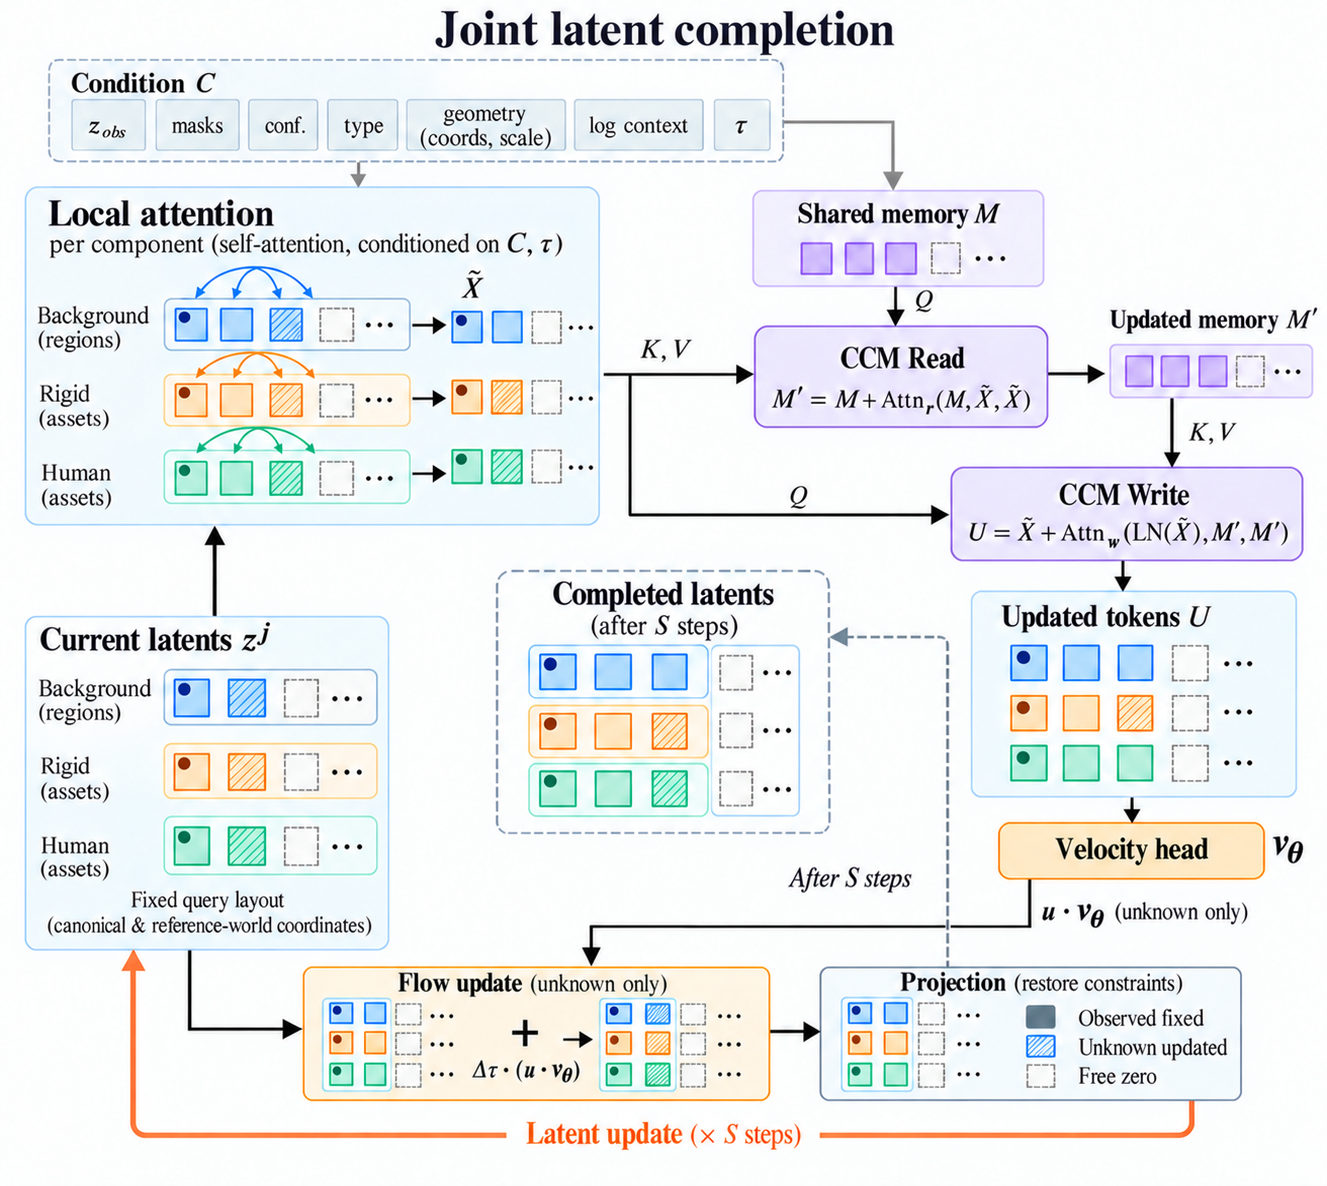
\includegraphics[width=0.86\textwidth]{../fig/drivecompose-joint-completion.png}
\caption{Enlarged version of the main joint-completion diagram. CCM reads group-local features into shared memory and writes context back. The velocity head and projection update unknown codes while restoring observed codes and clearing free-space codes.}
\label{fig:supp-detail}
\end{figure*}

\FloatBarrier
{\small
\bibliographystyle{ieeenat_fullname}
\bibliography{references}
}
\end{document}
